\documentclass[11pt]{beamer} 
\usetheme{cwc} 

\usepackage{amsmath,amssymb}
\usepackage{graphicx,acronym,setspace,epstopdf,pdflscape}
\usepackage{subeqnarray,multirow,cite,array,color,mathtools,setspace,geometry}

\acrodef{MSE}{mean squared error}
\acrodef{IBC}{interference broadcast channel}
\acrodef{MC}{multi-cell}
\acrodef{BS}{base station}
\acrodef{MIMO}{multiple-input multiple-output}
\acrodef{SISO}{single-input single-output}
\acrodef{MU}{multiple users}
\acrodef{OFDM}{orthogonal frequency division multiplexing}
\acrodef{WSRM}{weighted sum rate maximization}
\acrodef{QoS}{quality of service}
\acrodef{SCA}{successive convex approximation}
\acrodef{SNR}{signal-to-noise ratio}
\acrodef{MMSE}{minimum \acl{MSE}}
\acrodef{SIR}{signal-to-interference ratio}
\acrodef{SINR}{signal-to-interference-plus-noise ratio}
\acrodef{Q-WSRM}{queue \acl{WSRM}}
\acrodef{QM}{queue minimizing}
\acrodef{SRA}{spatial resource allocation}
\acrodef{JSFRA}{joint space-frequency resource allocation}
\acrodef{WMMSE}{weighted \acl{MMSE}}
\acrodef{KKT}{Karush-Kuhn-Tucker}
\acrodef{GP}{geometric programming}
\acrodef{SOC}{second-order cone}
%\acrodef{BCDM}{block coordinate descent method}
\acrodef{ADMM}{alternating directions method of multipliers}
\acrodef{PD}{primal decomposition}
\acrodef{DD}{dual decomposition}
\acrodef{FFR}{fractional frequency reuse}
\acrodef{DC}{difference of convex}
\acrodef{Q-WSRME}{\ac{Q-WSRM} extended}
\acrodef{TDD}{time division duplexing}
\acrodef{CSI}{channel state information}
\acrodef{AO}{alternating optimization}
\acrodef{OTA}{over-the-air}
\acrodef{PL}{path loss}
\acrodef{TDM}{time division multiplexing}
\acrodef{UC}{uncoordinated}
\acrodef{SoC}{system-on-chip}
\acrodef{WMMSE}{weighted minimum mean squared error}
\acrodef{AMBA}{Advanced Microcontroller Bus Architecture}
\acrodef{AXI}{Advanced Extensible Interface}
\acrodef{FPGA}{Field-programmable gate array}
\acrodef{MSMCSRAM}{multi-core shared memory}
\acrodef{IPC}{inter-processor communications}
\acrodef{CIC}{chip-level interrupt controller}
\acrodef{MCSDK}{multi-core software development kit}
\acrodef{AMP}{Asymmetric Multi-Processing}
\newcommand{\mbf}[1]{\mathbf{#1}}
\newcommand{\me}[1]{\( #1 \)}
\newcommand{\mc}[1]{\mathcal{#1}}
\newcommand{\fall}{\forall}
\newcommand{\set}[1]{\left \lbrace #1 \right \rbrace }
\newcommand{\mvec}[2]{\mathbf{#1}_{#2}}
\newcommand{\ith}[1]{{#1}^\mathrm{th}}
\newcommand{\pr}[1]{{#1}^\prime}
\newcommand{\mbfa}[1]{{\boldsymbol{#1}}}
\newcommand{\herm}{\mathrm{H}}
\newcommand{\sset}[1]{\left [ #1 \right ]}
\newcommand{\rfrac}[2]{{}^{#1}/{}_{#2}}
\newcommand{\eqspace}{\IEEEeqnarraynumspace}
\newcommand{\enoise}{\widetilde{N}_0}
\newcommand{\eqsub}{\IEEEyessubnumber}
\newcommand{\review}[1]{{\textcolor[rgb]{0 0 0.6}{#1}}}
\newcommand{\trace}{\mathrm{tr}}
\newcommand{\tran}{\mathrm{T}}
\newcommand{\R}[1]{\label{#1}\linelabel{#1}}
\newcommand{\lr}[1]{page~\pageref{#1}, line~\lineref{#1}}
\newcommand{\eqn}[1]{\(#1\)}
\newcommand{\mx}{\mbf{m}}
\newcommand{\my}{\mbf{w}}
\newcommand{\mz}{\mbfa{\gamma}}
\newcommand{\mxb}{{{\mbf{m}}}}
\newcommand{\myb}{{{\mbf{w}}}}
\newcommand{\iterate}[2]{{#1}^{(#2)}}
\newcommand{\iter}[3]{{#1}_{#2}^{(#3)}}
\newcommand{\ma}{\mbf{x}}

\graphicspath{{./../Figures/}}
\DeclareGraphicsExtensions{.pdf}

\epstopdfsetup{update,prepend,prefersuffix=false,suffix=}
\DeclareGraphicsRule{.eps}{pdf}{.pdf}{`epstopdf #1}
\pdfcompresslevel=9

\linespread{1.1}
\title{Implementation of MU-MIMO Schedulers on SoC}
\author{{Ganesh Venkatraman, Janne Janhunen, and Markku Juntti} \\ \scriptsize{Email: \{gvenkatr, janne.janhunen, markku.juntti\}@ee.oulu.fi}}

\begin{document}

\begin{frame}
    \titlepage
\end{frame}

\begin{frame}{Outline} \scriptsize
    \tableofcontents
\end{frame}

\acused{BS} \acused{MIMO} \acused{OFDM}

\section{Abstract}

\begin{frame}{Abstract}
	\begin{itemize}
		\item \blutxt{Problem Studied - } Implementing multi-user MIMO scheduler schemes on ZYNQ ZC702 SoC
		\item \blutxt{Issues addressed -}
			\begin{itemize}
				\item Complexity involved in implementing scheduling algorithms - \redtxt{low complex algorithm design}
				\item How to \redtxt{partition processing subsystem (PS) and programming logic (PL)} in ZYNQ SoC for implementing scheduler algorithms
			\end{itemize}
		\item \blutxt{Summary - } Proposed implementation \redtxt{supports up to \eqn{50} users in the system with \eqn{4 \times 4} MIMO configuration}
	\end{itemize}
\end{frame}

\section{Introduction}

\begin{frame}{Introduction and Motivation}
\begin{itemize}
\item Current standards are moving towards multi-antenna systems due to its numerous advantages
\item To avail the benefits, spatially multiplexing multiple user streams are considered
\item In order to do so, efficient precoding and user subset are to be identified
\item In this work, we analyze the computational needs of different MU-MIMO scheduling algorithms for a single scheduling block
\item We evaluate algorithm complexity with ZYNQ ZC702 SoC
\end{itemize}
\end{frame}

\section{System Model \& Assumptions}

\begin{frame}{Notations used}
\begin{itemize}
\item We consider a single-cell multi-user \ac{MIMO} scenario
\item Let \me{N_K} be the total number of users with \me{N_R} antenna elements
\item Let \me{\kappa} be the total available spatial streams for a user \me{k}, given by \me{\kappa = \min (N_T,N_R)}
\item \eqn{\mvec{H}{\hat{k}} \in \mathbb{C}^{N_R \times N_T}} be the channel between \ac{BS} and user \eqn{\hat{k}, \forall k \in \mc{U}}
\item Let \eqn{\mc{A} \subset \mc{U}} be the subset of users chosen by scheduling algorithm
\end{itemize}
\end{frame}

\begin{frame}{System Model}
\begin{itemize}
\item Let \eqn{\mvec{H}{\hat{k}} = \mvec{U}{\hat{k}} \mvec{D}{\hat{k}} \mvec{V}{\hat{k}}^\herm} be singular value decomposition of \eqn{\mvec{H}{\hat{k}}}
\item Let \eqn{k = \kappa \hat{k} + i} be the virtual user corresponding to the spatial stream \eqn{i \in \{0,\dotsc,\kappa-1\}}
\item Using this, we denote virtual channel \eqn{\mvec{h}{k} = \mvec{U}{\hat{k}}(i)^\herm \mvec{H}{\hat{k}}}, where \eqn{\mvec{U}{\hat{k}}(i)} corresponds to the column \eqn{i} of \eqn{\mvec{U}{\hat{k}}}
\item Now, the received symbol \eqn{\hat{d}_k} of virtual user \eqn{k} is given as
\[\hat{d}_k = \mvec{h}{k} \mvec{m}{k} d_k + \sum_{i \in \mc{A} \backslash \{k\}} \mvec{h}{k} \mvec{m}{i} d_i + {n}_{k}\]
\item where \me{\mvec{m}{k} \in \mathbb{C}^{N_T \times 1}} is the transmit precoder of user \me{k}
\end{itemize}
\end{frame}

\section{Scheduling Algorithms}

\begin{frame}{Overview of Scheduling Algorithms}
\begin{itemize}
	\item To minimize interference, only a subset of users are allowed for transmission
	\item Subset selection with certain objective requires exhaustive search
	\item \redtxt{Scheduling can inherently be performed by precoder designs} - efficient iterative algorithms are available
	\item However, as the user count increases, complexity scales up significantly
	\item Hence, precoders are to be designed only for a subset of users chosen by scheduling algorithms
\end{itemize}
\end{frame}

\subsection{Successive Projections}

\begin{frame}{Successive Projections\eqn{^\dagger}}
\begin{itemize}
\item Based on \redtxt{Gram-Schmidt Orthogonalization} Procedure
\item In each iteration, user channel vectors are projected on to the subspace orthogonal to the span of channel vectors already chosen
\item Upon \blutxt{projecting on to the orthogonal subspace}, resulting vector with maximum norm is chosen as the candidate user
\[\mbf{N}(\mathcal{A}) = \mbf{I}_{N_T} - \mbf{F} \left (\mbf{F}^\herm \mbf{F} \right )^{-1} \mbf{F}^\herm\]
\item where \eqn{\mbf{F}} is the matrix formed by stacking channel vector of already chosen users in \eqn{\mc{A}}
\end{itemize}
\eqn{^\dagger}\scriptsize{T. Yoo and A. Goldsmith, "{On the Optimality of Multi-Antenna Broadcast Scheduling using zero-forcing Beamforming},” in \emph{IEEE J. Sel. Areas Commun.}, vol. 24, no. 3. IEEE, march 2006.}
\end{frame}

\subsection{Product of Independent Projections}

\begin{frame}{Product of Independent Projections (PIPD)\eqn{^\dagger}}
	\begin{itemize}
	\item As compared to the subspace projection in previous algorithm, \blutxt{vector projections} are considered
	\item Each user channel is projected on to unit vector in the direction of already chosen users channel
	\item Selection is based on the product of independent vector projections
	\item Performs significantly closer to successive projections method
	\item Due to vector projections, inverse calculation is not required - \redtxt{low complexity}
	\end{itemize}
\eqn{^\dagger}\scriptsize{Venkatraman, G., Tolli, A., Janhunen, J., and Juntti, M. "Low Complexity Multi-User MIMO Scheduling for Weighted Sum Rate Maximization", in \emph{Proc. of European Signal Process. Conference (EUSIPCO)}, pp. 820--824, 2013}
\end{frame}

\subsection{Performance Figures}

\begin{landscape}
\begin{frame}[plain]
	\begin{figure}
		\centering
		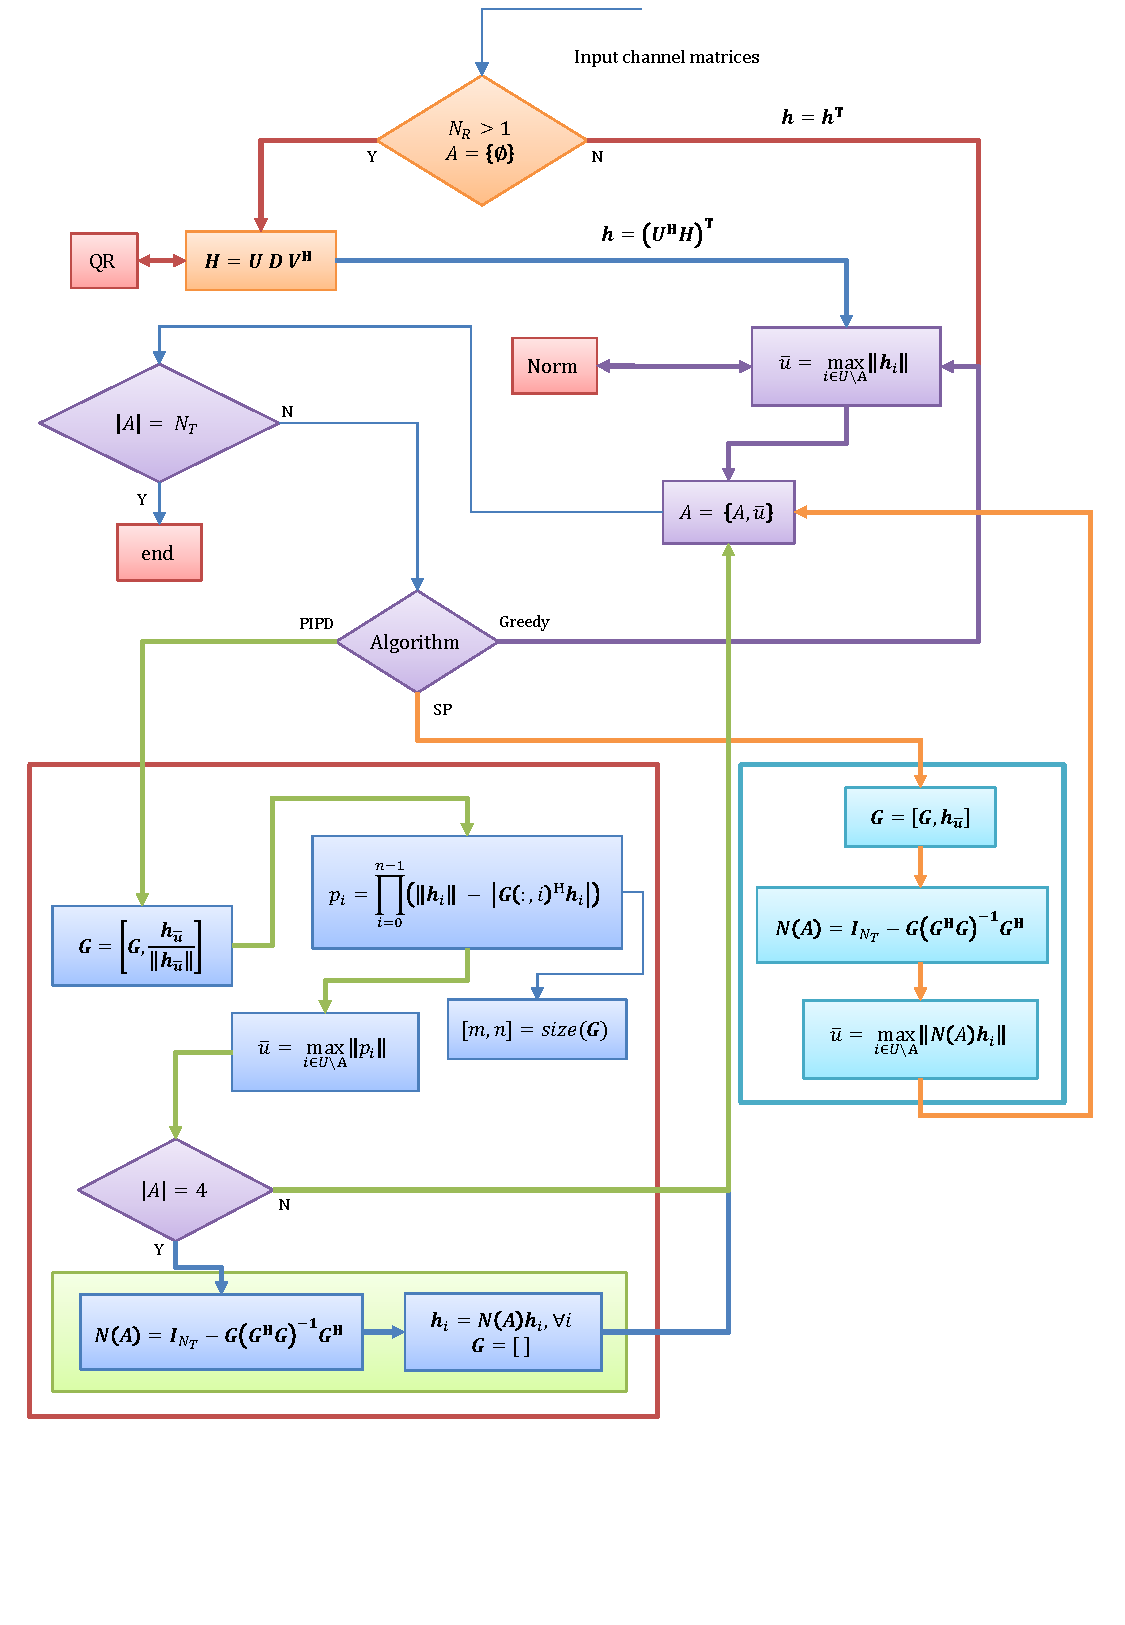
\includegraphics[trim=0.5in 1.5in 0in 1in,width=\columnwidth, angle=0]{Algorithm_Model}
		\caption{Block diagram of the scheduler algorithms: greedy, PIPD and successive projections}
	\end{figure}
\end{frame}
\end{landscape}

\begin{frame}
\begin{figure}
	\centering
	\caption{Comparison of Scheduler Algorithms for $N_K = 50$ users.}
	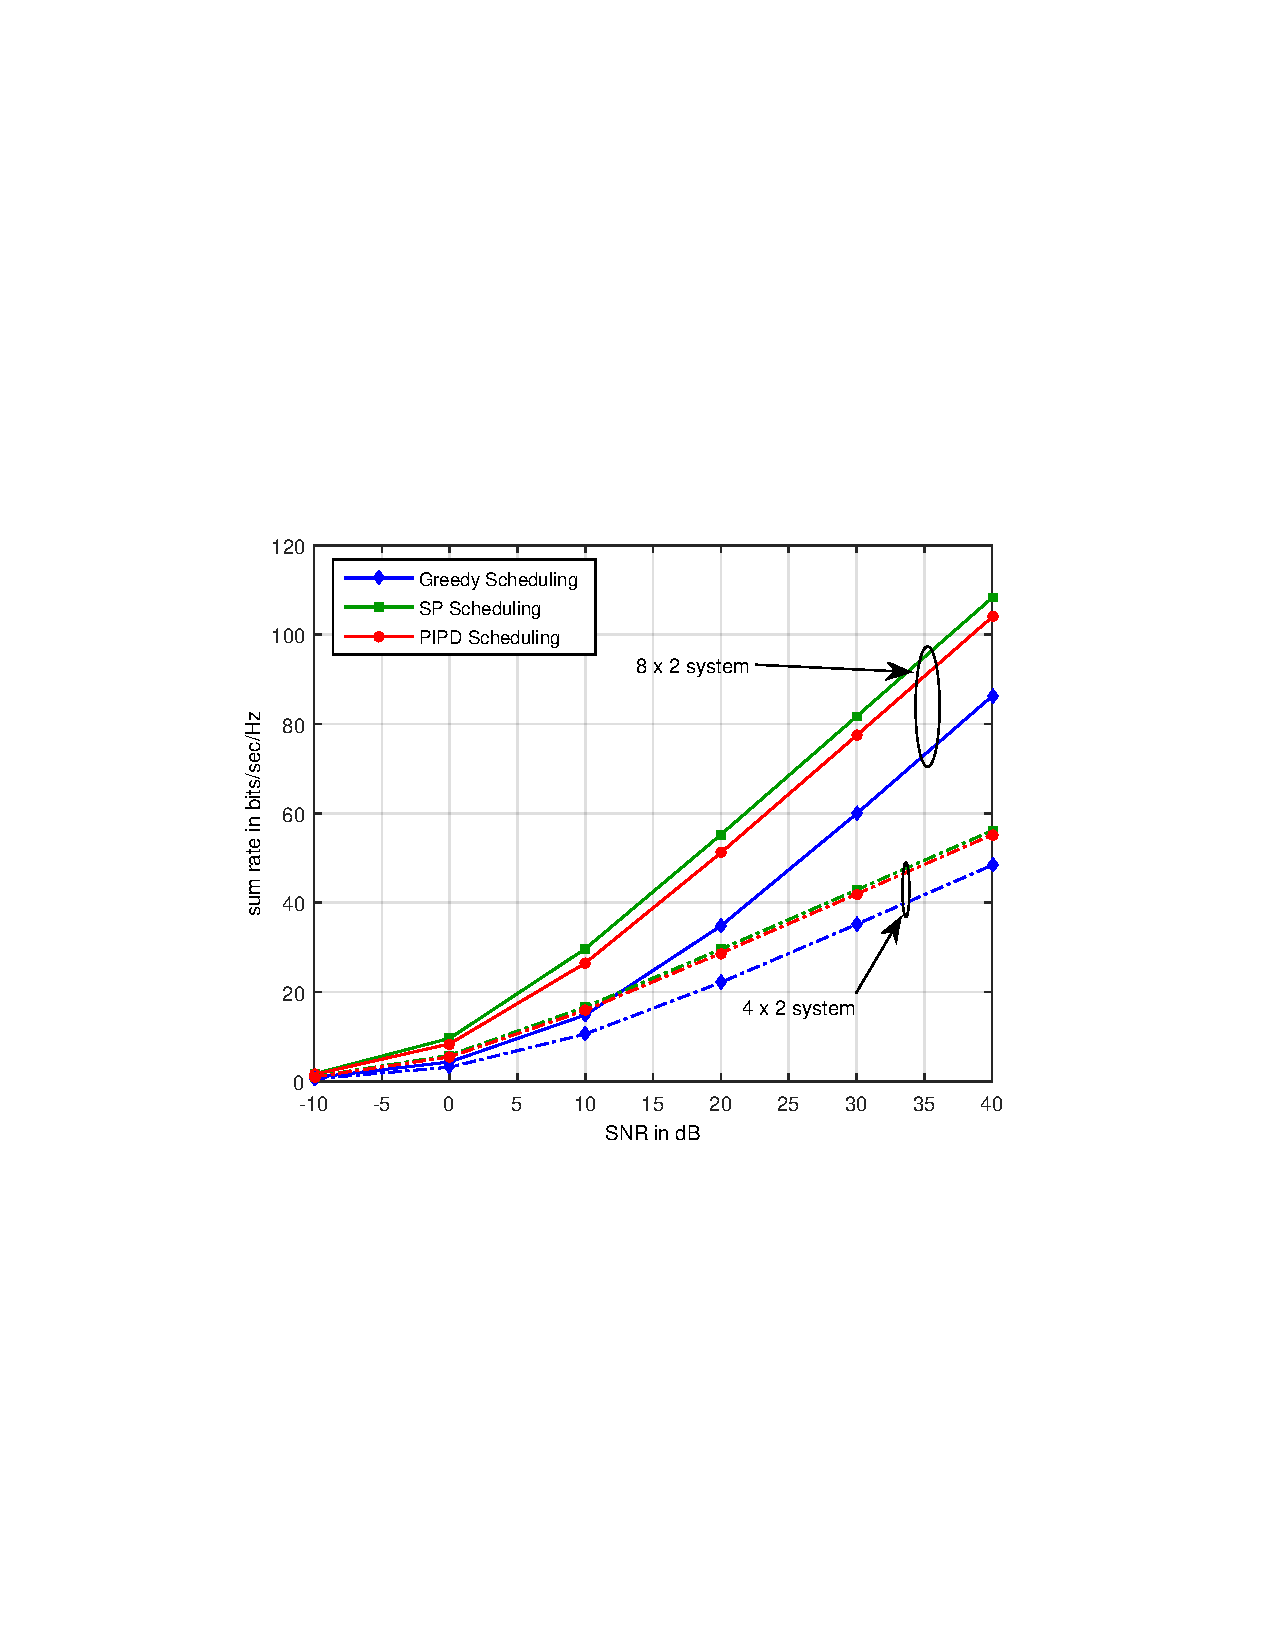
\includegraphics[trim=1.5in 3.5in 1.5in 3.5in,width=0.8\columnwidth]{sra_50_users}

\end{figure}
\end{frame}

\section{ZYNQ Implementation}

\subsection{Overview of ZYNC ZC702 SoC}

\begin{frame}{Overview of ZYNQ ZC702 SoC}
	\begin{itemize}
		\item ZC702 is a SoC, which includes \redtxt{dual core ARM Cortex A9 and FPGA}
		\item It supports AMBA-AXI interface between processing subsystem (PS) and programming logic (PL)
		\item \blutxt{Clock of ARM is $667$ MHz and PL operates at $100$ MHz}
		\item 1GB DDR RAM is accessible by both subsystems through AMBA-AXI
		\item Modes of communication between PS and PL can be
		\begin{itemize}
			\item B-RAM (block RAM)
			\item \blutxt{M\_AXI (burst transfer mode)}
			\item S\_AXI (streaming mode of transfer)
			\item S\_AXI\_Lite (address followed by data)
		\end{itemize}
	\end{itemize}
\end{frame}

\begin{frame}{Algorithm Partitioning}
	\begin{itemize}
		\item Computationally, SVD is the most demanding operation
		\item SVD is performed by repeated QR factorization (16 iterations)
		\item In order to utilize the SoC efficiently, \redtxt{SVD is performed in PL}
		\item Since PL operates at \eqn{100} MHz, we require parallel SVD operations to increase throughput
		\item With the available resources, only \blutxt{\eqn{5} SVD operations can be performed in parallel}
		\item Interface between \blutxt{PL and DDR is with \eqn{HP0} interconnect} - high performance AXI\_M mode
	\end{itemize}
\end{frame}

\begin{frame}{FPGA Resource Utilization for $5$ SVD's}
	\linespread{1.5}
	\begin{table} 
		 \begin{center} \small \begin{tabular}{|m{1.5in} m{1.5in}|} \hline
				\alert{Resource} 	&  	\alert{Utilization} \% \\ 
				\hline 
				Flip Flops 	& 	39.4 \\
				LUT 		& 	72.6 \\
				Memory LUT 	& 	6.2 \\
				BRAM 		& 	60.7 \\
				\blutxt{DSP48} 		& 	\blutxt{86.4 (limiting resource)}\\
				BUFG 		& 	3.1 \\ 
				\hline
			\end{tabular} \label{tbl-utilization} 
			\end{center} 
			\end{table}
\end{frame}

\begin{frame}
	\begin{figure}
		\centering
		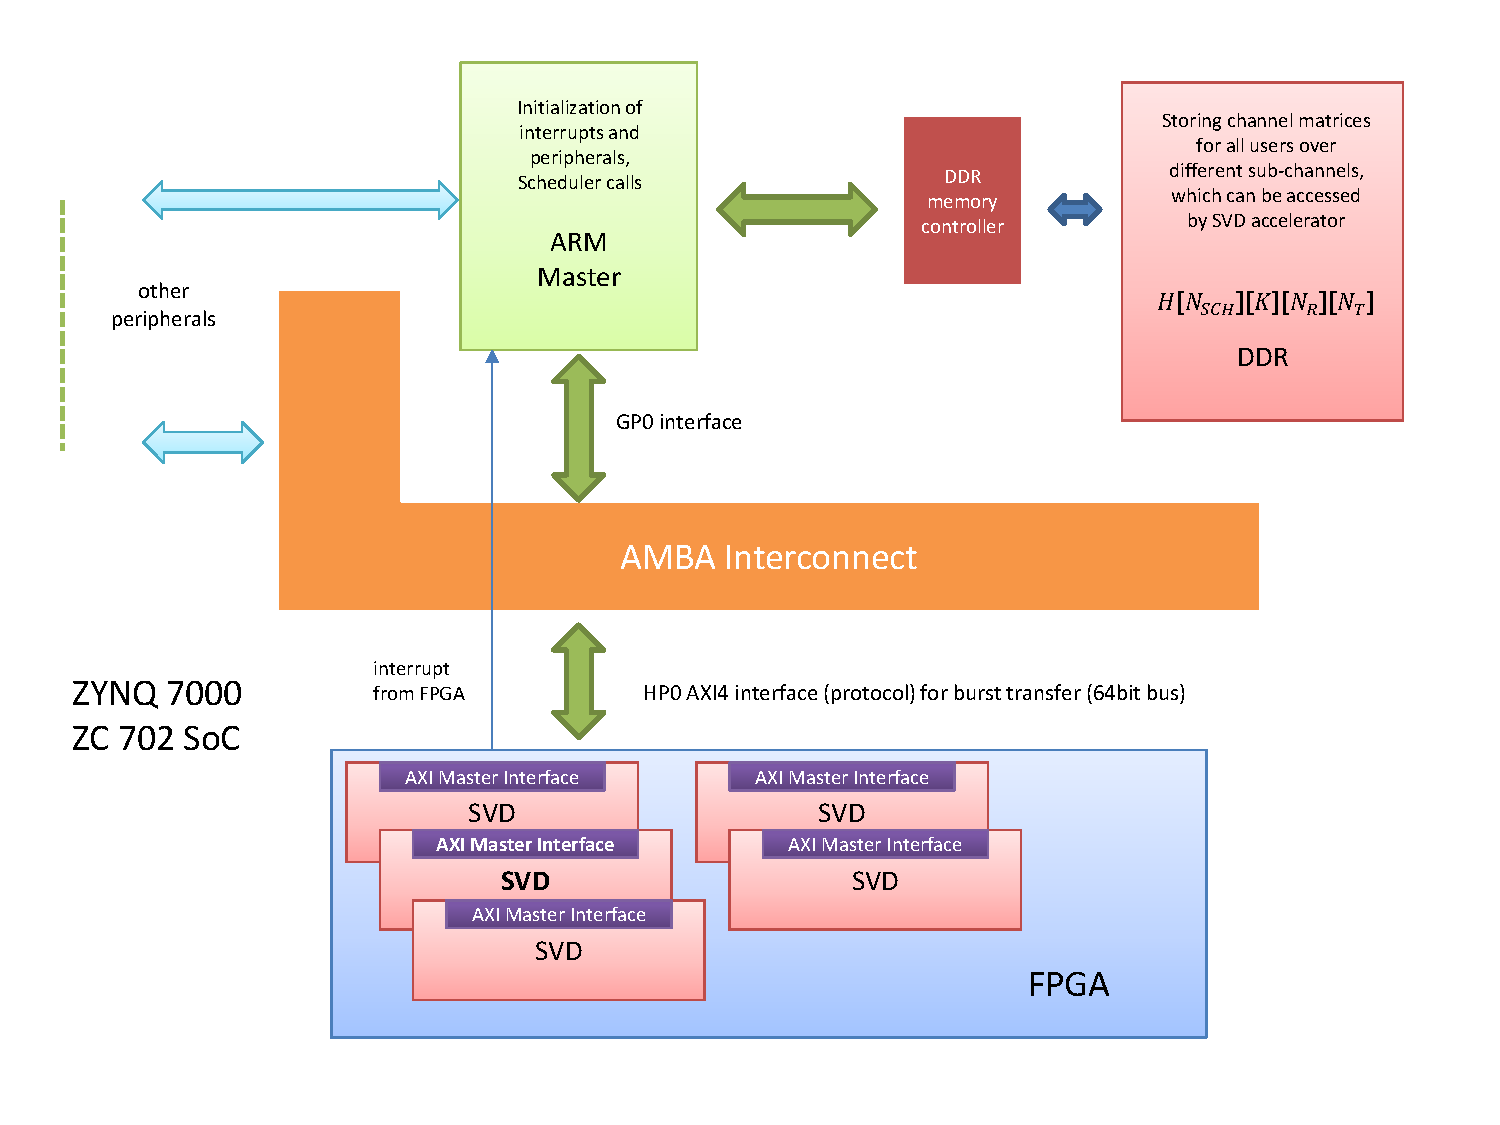
\includegraphics[trim=.75in .75in .75in .0in,width=0.8\columnwidth]{blk_diag}
		\caption{Software and Hardware Partitioning on ZYNQ 7ZC702}
	\end{figure}
\end{frame}

\subsection{PL-PS Implementation Specifications}

\begin{frame}{Why Scheduler Implementation on ARM}
	\begin{itemize}
		\item SVD is highly complex compared to scheduling complexity
		\item \blutxt{Scheduling is sequential}, \textit{i.e.}, users are selected based on previous chosen users
		\item However, metric calculation for all users and max search over all metrics can be done in parallel
		\item To do parallel implementation on PL, \redtxt{it requires more resources}, which we are lacking
		\item Similar parallelization can also be performed using \blutxt{NEON vector floating point (VFP) co-processor on ARM}
		\item SVD is required \blutxt{only when channel changes}, whereas \redtxt{scheduling is need on per sub-frame} basis
	\end{itemize}
\end{frame}


\begin{frame}{Programming Logic Implementation}
	\begin{itemize}
		\item Real and complex entries - \redtxt{Q3.15 signed format} 
		\item Dynamic range is improved by storing intermediate values in Q9.15
		\item Using above Q format, each \blutxt{MAC requires one {DSP48} unit}, \textit{i.e.} \eqn{25 \times 18} multiplication
		\item S\_AXI\_Lite is used for control command from PS \eqn{\to} PL, \blutxt{HP0 dedicated lane is used for fetching} from DDR
		\item Computes SVD for \redtxt{\eqn{5} channel matrices in parallel} to improve throughput
		\item Upon completion, an \blutxt{interrupt is sent to PS}
	\end{itemize}
\end{frame}

\begin{frame}{Processing Subsystem Implementation}
	\begin{itemize}
		\item \redtxt{Signed Q1.15 format} is used to represent real and imaginary entries
		\item Upon availability of channel, \blutxt{S\_AXI\_Lite control is used to interrupt PL for SVD}
		\item On obtaining interrupt from PL, a single ARM core is used to perform scheduling
		\item If there are multiple sub-channels, it can be performed over other ARM cores too
	\end{itemize}
\end{frame}

\subsection{Complexity Analysis}

\begin{frame}
\begin{table} \caption{Computational Complexity for one SB with $N_K = 50$ users} \begin{center} 
		\begin{tabular}{c c c c c c}
			\multirow{2}{*}{$N_T \times N_T $} & $\lambda$ & SVD Comp. & Greedy   & SP          & PIPD \\ 
			& streams & \eqn{\mathrm{msec}} & \eqn{\mathrm{msec}} & \eqn{\mathrm{msec}} & \eqn{\mathrm{msec}} \\
			\hline \\
			$8 \times 4$ & 4 & 11.427 & 0.098 & 2.029 & 1.280 \\ 
			$8 \times 4$ & 2 & 11.427 & 0.084 & 1.202 & 0.743 \\
			$8 \times 2$ & 2 & 3.231 & 0.079 & 1.225 & 0.704 \\
			$8 \times 2$ & 1 & 3.231 & 0.072 & 0.796 & 0.421 \\
			\hline \\
			$4 \times 4$ & 4 & 5.169 & 0.052 & 0.327 & 0.237 \\ 
			$4 \times 4$ & 2 & 5.170 & 0.042 & 0.189 & 0.168 \\
			$4 \times 2$ & 2 & 1.481 & 0.038 & 0.202 & 0.139 \\
			$4 \times 2$ & 1 & 1.481 & 0.033 & 0.131 & 0.089 \\
			\hline \vspace{-0.3in}
		\end{tabular} \label{table:compexity_comparison}\end{center}\end{table}
\end{frame}

\begin{frame}{Conclusion from Implementation Results}
	\begin{itemize}
		\item SVD is the computationally expensive part of scheduling
		\item However, due to channel coherency, SVD computation is not per subframe resolution
		\item Current implementation can perform \eqn{4,375} SVD's per second of \eqn{8 \times 4} matrix
		\item Similarly it can handle \eqn{33,760} SVD's per second of \eqn{4 \times 2} matrix
		\item All scheduling schemes satisfy real-time requirement of \eqn{1}msec with \eqn{4 \times 2} system with \eqn{N_K = 50} users
	\end{itemize}
\end{frame}


\section{Conclusions}

\begin{frame}{Conclusions}
\begin{itemize}
\item We studied the implementation of different state-of-the-art MU-MIMO scheduling algorithms on ZYNQ ZC702 SoC
\item Complexity is mainly attributed to SVD decomposition of channel matrices
\item Using parallel implementation, the overall throughput of SVD computation is improved \eqn{\approx 4.7} times \redtxt{(loss is due to memory bottleneck)}
\item We have demonstrated that with the current implementation, \blutxt{all scheduling schemes meet the real-time requirements}
\item As a comparative study, implementing above algorithms on \blutxt{TI C66K2H12 octa-core SoC}, supports up to \redtxt{$100$ users} for \eqn{4 \times 4} MIMO system (\gretxt{to appear in GlobalSIP 2015})
\end{itemize}
\end{frame}

\end{document}
